\documentclass[a4paper,11pt]{scrartcl}
\usepackage{graphicx}
\usepackage[utf8]{inputenc} 
\usepackage{amsmath,amssymb,amsthm} 
\usepackage[square, numbers]{natbib}
\usepackage{url}
\usepackage{xspace}
\usepackage[left=20mm,top=20mm]{geometry}
\usepackage{algorithmic}
\usepackage{subcaption}
\usepackage{mathpazo}
\usepackage{booktabs}
\usepackage{hyperref}

\newcommand{\ie}{i.e.}
\newcommand{\eg}{e.g.}
\newcommand{\reffig}[1]{Figure~\ref{#1}}
\newcommand{\refsec}[1]{Section~\ref{#1}}

\setcapindent{1em} %-- for captions of Figures

\renewcommand{\algorithmicrequire}{\textbf{Input:}}
\renewcommand{\algorithmicensure}{\textbf{Output:}}

\title{CPU-to-FPGA network offload engine}
\subtitle{Final Year Project Proposal}
\author{Patrick Wu\\ \url{patrick.wu.17@ucl.ac.uk}}
\date{14 Oct, 2020}

\begin{document}

\maketitle

\section{Project Context}
Networking applications are becoming increasingly demanding due to the huge increase in the amount of data generated nowadays. More and more, these applications require higher bandwidth and lower latency to archive better and more responsive service. Hence, it is becoming a challenge not to overload the CPU with a network stack running at maximum bandwidth \cite{chen-2018}. In other words, the CPU should be enabled to spend more of its resource dealing with actual data rather than running the network stacks.

DPU-based NICs (Data Processing Unit based Network Interface Cards) are designed to offload the traffic processing steps of the network stack from the CPU and the kernel \cite{mellanox}. Compared to simple NICs, DPU-based NIC goes beyond simple connectivity and implements network traffic processing on the board. Namely, network offloading NICs can be divided into 3 types, ASIC-based, FPGA-based and SOC-based, each with their own trade-offs \cite{mellanox}. As shown in Figure \ref{nic-comparison} below, an ASIC-Based NIC provides the best performance out of all 3, but the development cost is also the most expensive and the extensibility is the worst out of all 3. On the other side of the spectrum, SOC-based NIC requires the least development but the performance is incomparable with the other hardware-based solutions.
\begin{figure}[h]
    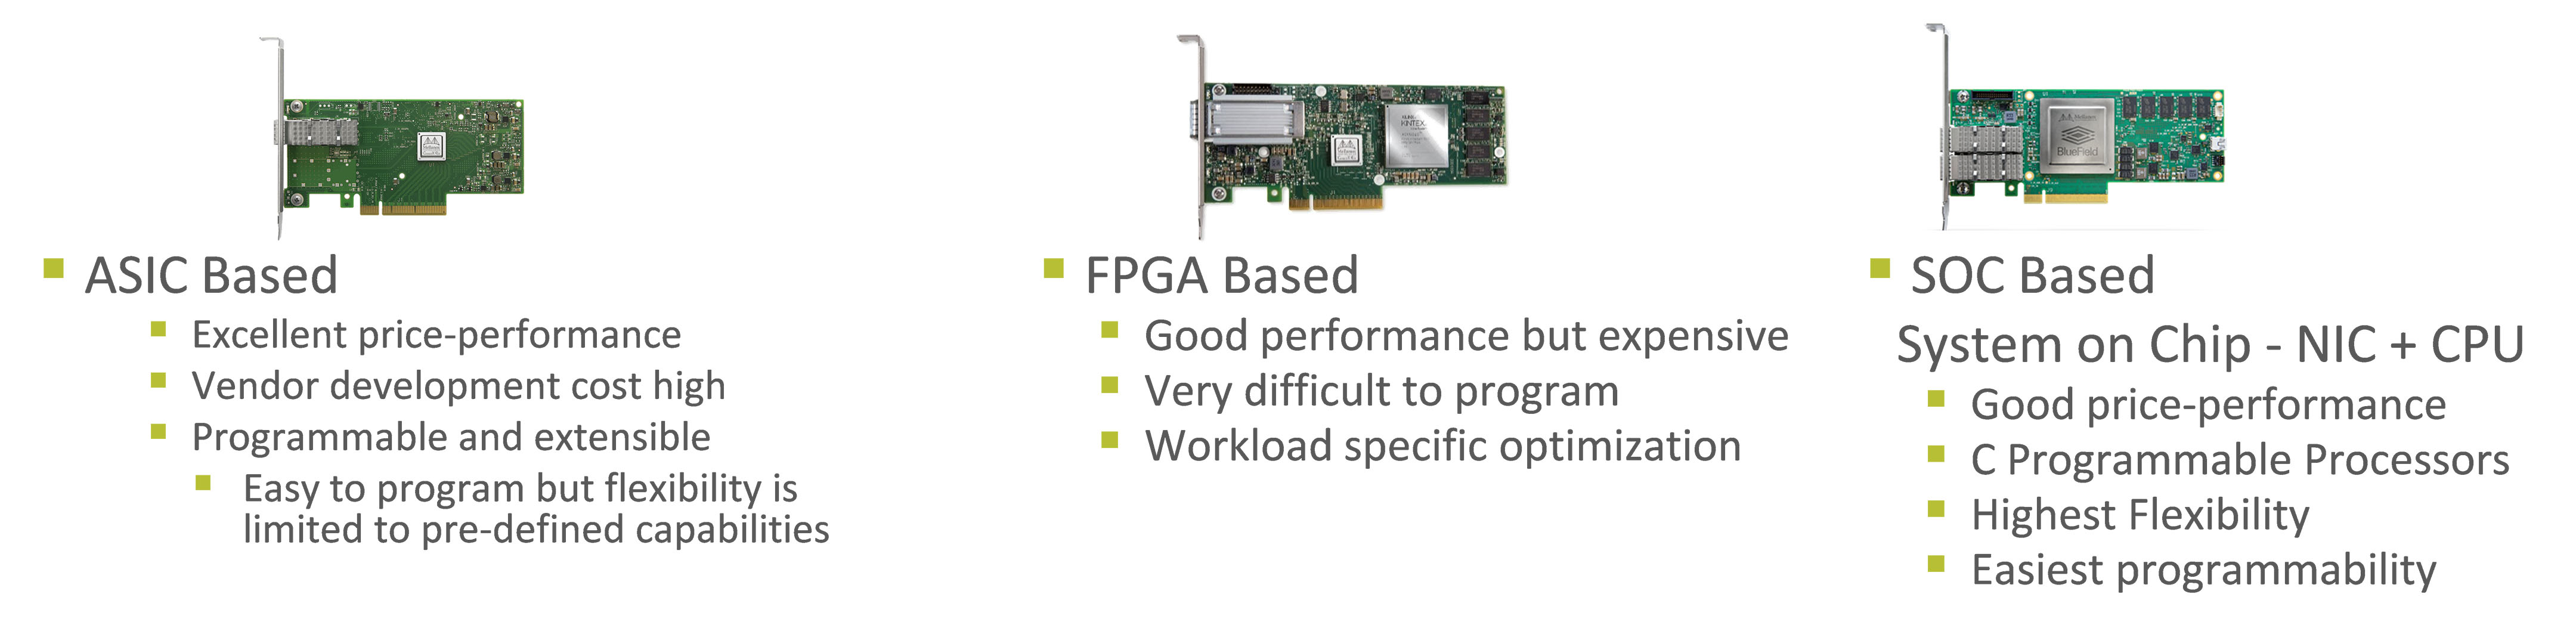
\includegraphics[width=\textwidth]{imgs/nic1-1.jpg}
    \caption{DPU-based NIC card comparison}
    \label{nic-comparison}
\end{figure}

Therefore, Field-Programmable Gate Arrays (FPGAs) has been proven to be a middle ground in this scenario. With their unique mix of configurable hardware logic, its NIC can deliver great network processing performance while keeping the development cost rather low. One can program an FPGA card simply by flashing a program on to the board, which is not possible compared to its ASIC counterparts \cite{4068926}.

Such that, the project aims to explore the possibility and usability of offloading lower layers of network connections to FPGAs. This includes building an offload engine that processes incoming network traffic on the board and exposing designed APIs for software to access processed application data.

\section{Project Overview}
\begin{figure}[h]
    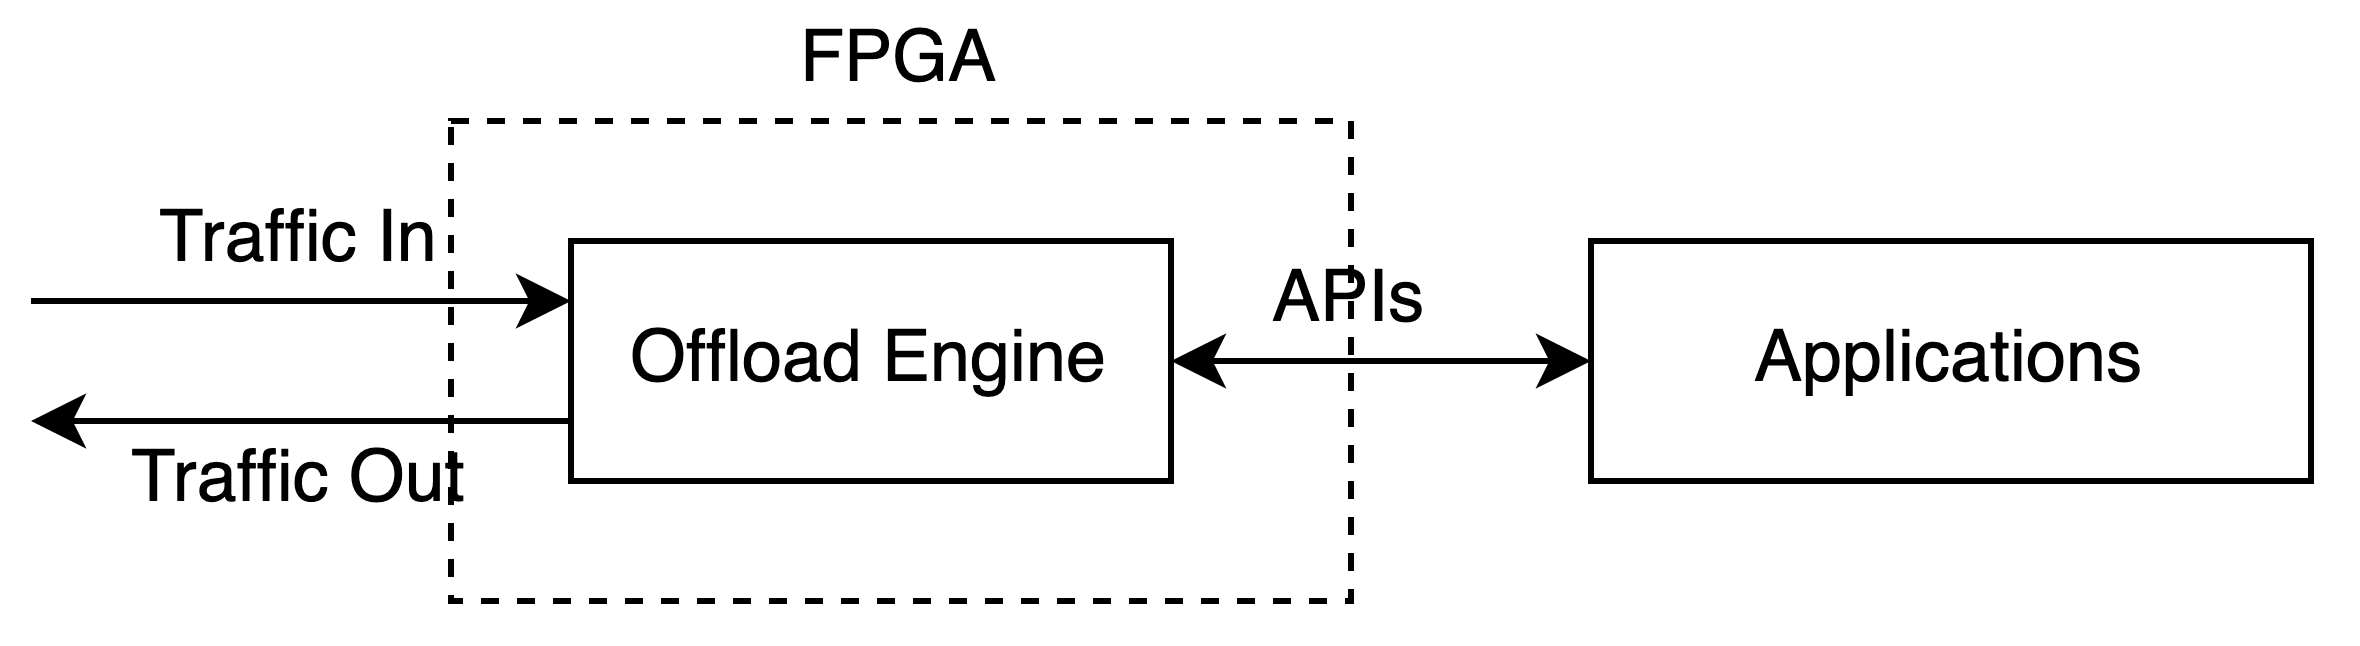
\includegraphics[width=\textwidth]{imgs/design.png}
    \caption{Design Overview}
    \label{design-overview}
\end{figure}

In this project, the main goal is to build an offload engine that handles Ethernet frames coming in and out of the node. The design of the project is shown above in Figure \ref{design-overview}. A Xilinx Spartan 3E Starter Kit with an RJ45 connector would be used to handle the traffic as an offload engine. Applications running on host computer connecting to the board via USB (subject to change) would be able to receive and send processed data through the network via the software interfaces provided on the board.

\section{Project Objectives}

\subsection{First Milestone}
\begin{itemize}
    \item To understand networking concepts, and implement senders and receivers of Ethernet packets via raw socket provided by the Linux Kernel
    \item To acquire knowledge used in FPGA programming, setup and understand FPGA development environment and write basic Verilog programs
\end{itemize}

\subsection{Second Milestone - Receive Packets}
\begin{itemize}
    \item To implement offload engine in FPGA that would handle packet receiving from the network
    \item To provide API for software to read processed packets
\end{itemize}

\subsection{Third Milestone - Send Packets}
\begin{itemize}
    \item To implement offload engine in FPGA that would handle packet sending to the network
    \item To provide API for software to send new packets
\end{itemize}

\subsection{Stretch Goals}
\begin{itemize}
    \item To develop an integrity checking framework to check packet validity
    \item To implement offload engine to handle ICMP, IP packets
    \item To implement offload engine to handle UDP/IP packets
    \item To provide more comprehensive APIs for applications upwards of Layer 3 running on UDP/IP stack
    \item TBD...
\end{itemize}

\bibliographystyle{unsrt}
\bibliography{proposal}

\end{document}